%%%%%%%%%%%%%%%%%%%%%%%%%%%%%%%%%%%%%%%
% Wenneker Resume/CV
% LaTeX Template
% Version 1.1 (19/6/2016)
%
% This template has been downloaded from:
% http://www.LaTeXTemplates.com
%
% Original author:
% Frits Wenneker (http://www.howtotex.com) with extensive modifications by 
% Vel (vel@LaTeXTemplates.com)
%
% License:
% CC BY-NC-SA 3.0 (http://creativecommons.org/licenses/by-nc-sa/3.0/
%
%%%%%%%%%%%%%%%%%%%%%%%%%%%%%%%%%%%%%%

%----------------------------------------------------------------------------------------
%	PACKAGES AND OTHER DOCUMENT CONFIGURATIONS
%----------------------------------------------------------------------------------------

\documentclass[a4paper,12pt]{memoir} % Font and paper size

%%%%%%%%%%%%%%%%%%%%%%%%%%%%%%%%%%%%%%%%%
% Wenneker Resume/CV
% Structure Specification File
% Version 1.1 (19/6/2016)
%
% This file has been downloaded from:
% http://www.LaTeXTemplates.com
%
% Original author:
% Frits Wenneker (http://www.howtotex.com) with extensive modifications by 
% Vel (vel@latextemplates.com)
%
% License:
% CC BY-NC-SA 3.0 (http://creativecommons.org/licenses/by-nc-sa/3.0/)
%
%%%%%%%%%%%%%%%%%%%%%%%%%%%%%%%%%%%%%%%%%

%----------------------------------------------------------------------------------------
%	PACKAGES AND OTHER DOCUMENT CONFIGURATIONS
%----------------------------------------------------------------------------------------

\usepackage{XCharter} % Use the Bitstream Charter font
\usepackage[utf8]{inputenc} % Required for inputting international characters
\usepackage[T1]{fontenc} % Output font encoding for international characters

\usepackage[top=1cm,left=1cm,right=1cm,bottom=1cm]{geometry} % Modify margins

\usepackage{graphicx} % Required for figures

\usepackage{flowfram} % Required for the multi-column layout

\usepackage{url} % URLs

\usepackage[usenames,dvipsnames]{xcolor} % Required for custom colours

\usepackage{tikz} % Required for the horizontal rule

\usepackage{enumitem} % Required for modifying lists
\setlist{noitemsep,nolistsep} % Remove spacing within and around lists

\setlength{\columnsep}{\baselineskip} % Set the spacing between columns

% Define the left frame (sidebar)
\newflowframe{0.2\textwidth}{\textheight}{0pt}{0pt}[left]
\newlength{\LeftMainSep}
\setlength{\LeftMainSep}{0.2\textwidth}
\addtolength{\LeftMainSep}{1\columnsep}
 
% Small static frame for the vertical line
\newstaticframe{1.5pt}{\textheight}{\LeftMainSep}{0pt}
 
% Content of the static frame with the vertical line
\begin{staticcontents}{1}
\hfill
\tikz{\draw[loosely dotted,color=RoyalBlue,line width=1.5pt,yshift=0](0,0) -- (0,\textheight);}
\hfill\mbox{}
\end{staticcontents}
 
% Define the right frame (main body)
\addtolength{\LeftMainSep}{1.5pt}
\addtolength{\LeftMainSep}{1\columnsep}
\newflowframe{0.7\textwidth}{\textheight}{\LeftMainSep}{0pt}[main01]

\pagestyle{empty} % Disable all page numbering

\setlength{\parindent}{0pt} % Stop paragraph indentation

%----------------------------------------------------------------------------------------
%	NEW COMMANDS
%----------------------------------------------------------------------------------------

\newcommand{\userinformation}[1]{\renewcommand{\userinformation}{#1}} % Define a new command for the CV user's information that goes into the left column

\newcommand{\cvheading}[1]{{\Huge\bfseries\color{RoyalBlue} #1} \par\vspace{.6\baselineskip}} % New command for the CV heading
\newcommand{\cvsubheading}[1]{{\Large\bfseries #1} \bigbreak} % New command for the CV subheading

\newcommand{\Sep}{\vspace{1em}} % New command for the spacing between headings
\newcommand{\SmallSep}{\vspace{0.5em}} % New command for the spacing within headings

\newcommand{\aboutme}[2]{ % New command for the about me section
\textbf{\color{RoyalBlue} #1}~~#2\par\Sep
}
	
\newcommand{\CVSection}[1]{ % New command for the headings within sections
{\Large\textbf{#1}}\par
\SmallSep % Used for spacing
}

\newcommand{\CVItem}[2]{ % New command for the item descriptions
\textbf{\color{RoyalBlue} #1}\par
#2
\SmallSep % Used for spacing
}

\newcommand{\bluebullet}{\textcolor{RoyalBlue}{$\circ$}~~} % New command for the blue bullets
 % Include the file specifying document layout and packages

%----------------------------------------------------------------------------------------
%	NAME AND CONTACT INFORMATION 
%----------------------------------------------------------------------------------------


\userinformation{ % Set the content that goes into the sidebar of each page
\begin{flushright}
% Comment out this figure block if you don't want a photo
%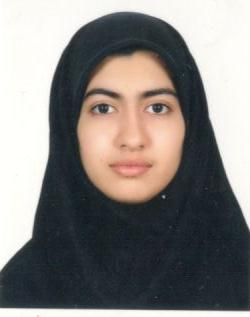
\includegraphics[width=0.6\columnwidth]{mahin.jpg}\\[\baselineskip] % Your photo
\small % Smaller font size
%Mahin Mirshams\\ % Your name
%\url{m.mirshams66@gmail.com} \\ % Your email address
%\url{m.mirshams@aut.ac.ir} \\ % Your URL
%\url{github.com/mahinmirshams} \\ % Your URL
\Sep % Some whitespace
\textbf{Contact} \\
+98 9195712281 \\ % Your phone number
\Sep % Some whitespace
\textbf{Email} \\
\url{m.mirshams66@gmail.com} \\
\url{m.mirshams@aut.ac.ir}  \\
\textbf{GitHub}\\
\url{https://github.com/mahinmirshams}
\vfill % Whitespace under this block to push it up under the photo
\end{flushright}
}


%----------------------------------------------------------------------------------------

\begin{document}
\footnotesize

\userinformation % Print your information in the left column

\framebreak % End of the first column

%----------------------------------------------------------------------------------------
%	HEADING
%----------------------------------------------------------------------------------------

\cvheading{Mahin Mirshams} % Large heading - your name

\cvsubheading{Computer Engineering Student} % Subheading - your occupation/specialization

%----------------------------------------------------------------------------------------
%	ABOUT ME
%----------------------------------------------------------------------------------------

\aboutme{About Me}{I was born in Esfahan. Spend the early years of my life in Moscow, Russia. Currently spending my time on my studying and working as a part-timer.}

%----------------------------------------------------------------------------------------
%	EDUCATION
%----------------------------------------------------------------------------------------

\CVSection{Education}

%------------------------------------------------

\CVItem{2015 - Current, AmirKabir University of Technology (Tehran Polytechnic), Tehran, Iran}{BS in Computer Engineering(IT). GPA:TBA/20}

%------------------------------------------------

\CVItem{2011 - 2015, Farzanegan3(NODET) High School, Tehran, Iran}{Diploma in Mathematics and Science.GPA: 19.43/20}

%------------------------------------------------




\Sep % Extra whitespace after the end of a major section

%----------------------------------------------------------------------------------------
%	EXPERIENCE
%----------------------------------------------------------------------------------------

\CVSection{Experience}

%------------------------------------------------


\CVItem{Current, \textit{software programmer of  ADCS, C\&DH}, Khaje Nasir Toosi University of Technology (KNTU) }{
A member of Attitude Determination and Control Subsystem of Space Research Lab K.N.Toosi University of Technology}

\CVItem{Winter 2018, \textit{Teaching Assistant}, Amirkabir University of technology }{
Advance Programming (Java)
}\\
\CVItem{Fall 2017, \textit{Teaching Assistant}, Amirkabir University of technology }{
Principle of Computer and C Programming  
}
\\
\CVItem{Summer 2016, \textit{Teaching Assistant}, Shariati University  }{
Java Programming Language 
%\begin{itemize}
%	\item Learned how to make amazing coffee
%	\item Finally determined the reason for \textsc{PC LOAD LETTER}:
	%\begin{itemize}
	%	\item Paper jam
		%\item Software issues:
		%\begin{itemize}
		%	\item Word not sending the correct data to printer
		%	\item Windows trying to print in letter format
		%\end{itemize}
		%\item Coffee spilled inside printer
%	\end{itemize}
%	\item Broke the office record for number of kitten pictures in cubicle
%	\item Learned how to make more amazing coffee on a new machine
%	\item Mastered the art of filing accurate TPS reports
%\end{itemize}
}
\\
\CVItem{Fall 2016, \textit{Teaching Assistant}, Amirkabir University of technology   }{
Principle of Computer and C Programming  
}
\\
\CVItem{summer 2016, \textit{C\&DH Programmer}, Amirkabir University of technology   }{
Spending internship as one of members of the AUTSAT project 
}
\\

%------------------------------------------------

%\CVItem{Jan 2008 - Oct 2012, \textit{Computer Repair Specialist}, Buy More}{Worked in the Nerd Herd and helped to solve computer problems by asking customers to turn their computers off and on again.}

%------------------------------------------------

 % Extra whitespace after the end of a major section

%----------------------------------------------------------------------------------------
%	COMMUNICATION SKILLS
%----------------------------------------------------------------------------------------
\CVSection{Communication Skills}

%------------------------------------------------

\CVItem{2017 - Current, \textit{Publish Magazine}, Student Guild Council of AmirKabir Computer Engineering Faculty }{Chief editor of Pouyesh Magazine as One the  members of Student Guild Council.}



\CVItem{2017, \textit{Oral Presentation}, Research and  Technical Presentation Course}{As part of the course work, Presented an Introduction To Satellite Control Software.}



%------------------------------------------------

\CVItem{2017, \textit{Oral Presentation}, First Summer Camp of the APSCO Student Small Satellite(SSS), China}{As part of the course assignment, I wrote an essay on Attitude and Determination Control Subsystems of Triple-S Micro Satellite which was presented at the end of the camp in English at Beihang University.}

%------------------------------------------------
\CVItem{2015, \textit{Oral Presentation}, Computer WorkShop Course }{As part of the course work, our group presented An Introduction to Latex Programming Language and using Xepersian Package.}

 % Extra whitespace after the end of a major section

%----------------------------------------------------------------------------------------
%	SKILLS
%----------------------------------------------------------------------------------------

\CVSection{Software Development Skills}

%------------------------------------------------

\CVItem{Programming}
{\begin{tabular}{p{0.2\textwidth} p{0.2\textwidth} p{0.2\textwidth}}
\bluebullet C/C++  &  \bluebullet Java & \bluebullet C{\#} \\
\bluebullet LaTex & \bluebullet HTML/CSS &  \bluebullet Microsoft Office \\
\bluebullet MySql/Postgresql & \bluebullet Verilog &
 \bluebullet Vhdl \\ \bluebullet Python & \bluebullet Matlab
\end{tabular}}

%------------------------------------------------

\CVSection{Language Skills}

%------------------------------------------------

\CVItem{}
{\begin{tabular}{p{0.7\textwidth} p{0.2\textwidth} p{0.2\textwidth}}
\bluebullet Persian(native speaker) \\\bluebullet English(Advance degree from Cavendish University Institute  in Tehran) \\  \bluebullet Chinese(beginner) \\

\end{tabular}}

%------------------------------------------------

%\CVItem{Computer Software}
%{\begin{tabular}{p{0.2\textwidth} p{0.2\textwidth} p{0.2\textwidth}}
 %\bluebullet MySQL &  \bluebullet iOS & \bluebullet Android\\
%\end{tabular}}

%------------------------------------------------

\Sep % Extra whitespace after the end of a major section

%----------------------------------------------------------------------------------------
%	NEW PAGE DELIMITER
%	Place this block wherever you would like the content of your CV to go onto the next page
%----------------------------------------------------------------------------------------

\clearpage % Start a new page

\userinformation % Print your information in the left column

\framebreak % End of the first column

%----------------------------------------------------------------------------------------
%	AWARDS
%----------------------------------------------------------------------------------------

\CVSection{Awards}

%------------------------------------------------

\CVItem{2013, \textit{ACM student contest},  Tehran Shekofa Festival}{Placed  2nd in the ACM student contest among  all the student in Tehran.}\\
\CVItem{2016, \textit{Amirkabir Programming League(APL)},   AmirKabir University of Technology (Tehran Polytechnic)}{participating as a contestant.}\\
\CVItem{2016, \textit{Mobile Programming Marathon},  Sharif University of Technology }{Placed  among the best 10  in the marathon among  all the participating groups.}\\
\CVItem{2017, \textit{ First Summer Camp of the APSCO Student Small Satellite(SSS) },  Beihang University of China }{Participated as Software Programmer of Attitude Determination and Control Subsystem (ADCS). Awarded as "Excellent Student".}
\\
\CVItem{2017, \textit{ BimeTech (BimeBazar Programming Marathon)},  Sharif University of Technology }{Placed  among the best 10  in the marathon among  all the participating groups. }
%------------------------------------------------
% Extra whitespace after the end of a major section

%----------------------------------------------------------------------------------------
%	INTERESTS
%----------------------------------------------------------------------------------------


\CVSection{Interests}

%------------------------------------------------

\CVItem{Professional}{  Software Design, Web Design, Data Base Design, ACM, Team Managing, Human Resource, Project Managing, Marketing }

%------------------------------------------------

\CVItem{Personal}{Foreign Language(Chinese), Sport(Professional Swimmer), Reading books, Playing Music (Piano), Astronomy }

%------------------------------------------------


%\CVSection{Position in SSS-1 project}

%------------------------------------------------


%\begin{tabular}{p{0.7\textwidth} p{0.2\textwidth} p{0.2\textwidth}}
%\bluebullet 
%software programmer of  ADCS  , C\&DH  \\



%\end{tabular}


\Sep % Extra whitespace after the end of a major section

%----------------------------------------------------------------------------------------

\end{document}
